\documentclass{beamer}
\usepackage{xcolor}
\usepackage{listings}
\usepackage{polyglossia}
\setmainlanguage{spanish}
\setmainfont
[Ligatures=TeX, % recommended
UprightFont={*},
ItalicFont={* Italic},
BoldFont={* Bold},
BoldItalicFont={* Bold Italic}]
{Fira Sans}
\setsansfont
[Ligatures=TeX, % recommended
UprightFont={*},
ItalicFont={* Italic},
BoldFont={* Bold},
BoldItalicFont={* Bold Italic}]
{Fira Sans}
\setmonofont{Fira Mono}
\newfontfamily\FiraTitle
[Ligatures=TeX, % recommended
UprightFont={* Heavy},
BoldFont={* Ultra}]
{Fira Sans}
\definecolor{green}{HTML}{4BCDAD}
\definecolor{purple}{HTML}{F173AE}

\title{\resizebox{\columnwidth}{!}{{\FiraTitle \textbf{\texorpdfstring{\textcolor{black}{Git}}{Git} \texorpdfstring{\color{green}{+}}{+} \texorpdfstring{\textcolor{purple}{Github}}{Github}}}}}
\subtitle{\resizebox{0.5\columnwidth}{!}{\FiraTitle \texorpdfstring{\textcolor{black}{De 0 a 100 en una clase}}{De 0 a 100 en una clase}}}
\institute{Universidad de Guanajuato}
\author{{\FiraTitle \texorpdfstring{\textcolor{black}{Mario Alejandro Gil Lázaro}}{Mario Alejandro Gil Lázaro}}}
\date{}

\setbeamercolor{frametitle}{fg=green}

\begin{document}

\frame{\titlepage}

\begin{frame}
  \frametitle{Tabla de contenidos}
  \tableofcontents
\end{frame}

\begin{frame}
  \frametitle{{\FiraTitle \textbf{Introducción: Sistemas de Control de Versiones}}}
  \begin{columns}
    \column{0.5\textwidth}
    {\FiraTitle Beneficios}
    \begin{itemize}
      \item Historial de cambios para todos los archivos
      \item Branching y merging
      \item Rastreabilidad
      \end{itemize}
    \column{0.5\textwidth}
    \begin{figure}
      \centering
      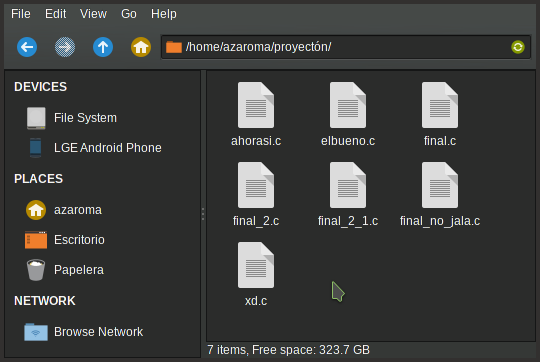
\includegraphics[width=\textwidth]{version}
      \caption{Control de versiones antiguo}
    \end{figure}
  \end{columns}
\end{frame}

\begin{frame}
\frametitle{¿Por qué Git?}
\begin{figure}
  \centering
  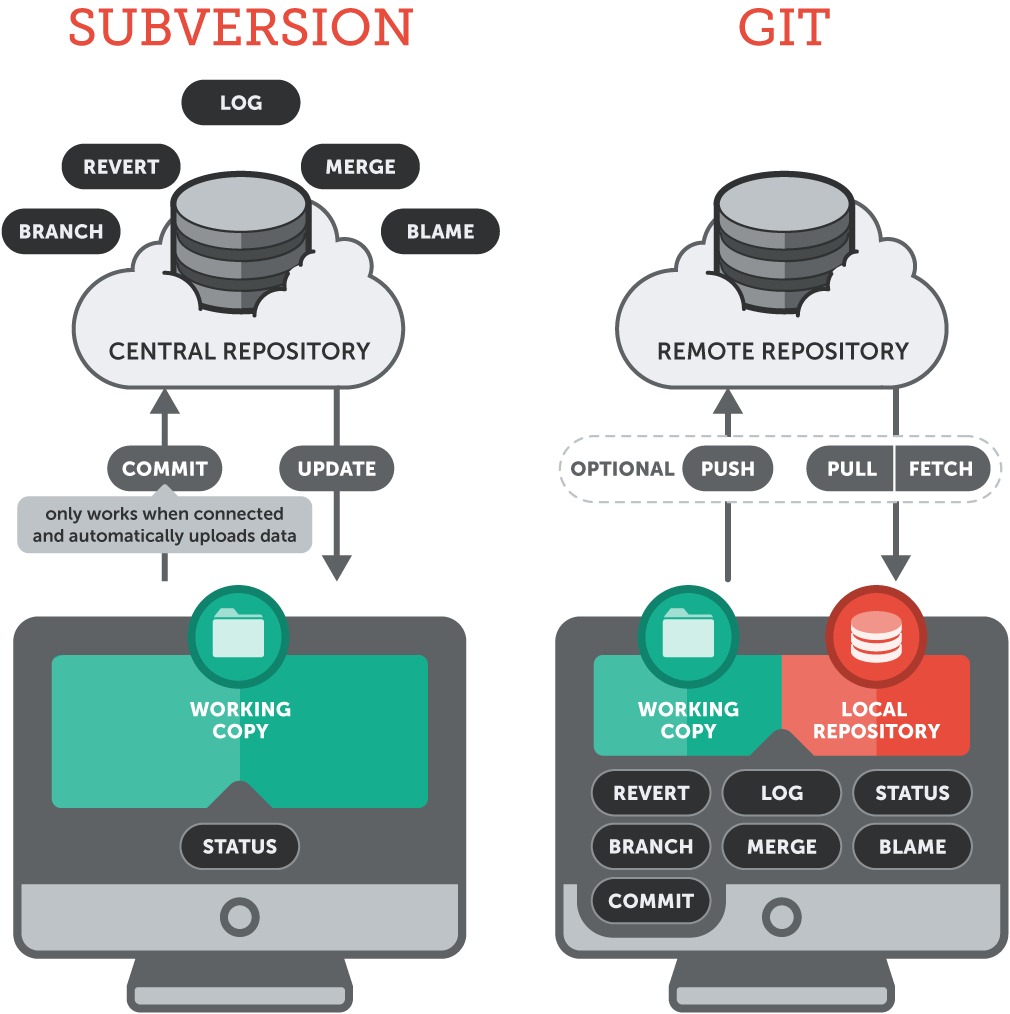
\includegraphics[scale=0.2]{centralizado-vs-distribuido}
  \caption{Diferencias entre un sistema de control de versiones distribuido y uno centralizado}
\end{figure}
\end{frame}

\begin{frame}
\frametitle{Repositorio}
Estructura de datos que almacena metadatos y/o un sistema de archivos.

\vspace{2em}

\colorbox{purple}{\lstinline|git init|} convierte el directorio actual en un repositorio.

\vspace{1em}

\colorbox{purple}{\lstinline°git clone <http|ftp|ssh>°} crea una copia local de un repositorio remoto.
\end{frame}

\begin{frame}
  \begin{center}
    \resizebox{\textwidth}{!}{\FiraTitle \color{green}{git status}}
    \resizebox{0.7\textwidth}{!}{\FiraTitle \color{purple}{git log}}
  \end{center}
\end{frame}

\begin{frame}
\frametitle{Add}
\end{frame}

\begin{frame}
\frametitle{.gitignore}
\end{frame}

\begin{frame}
\frametitle{Commit}
\end{frame}

\begin{frame}
\frametitle{Branch}
\end{frame}

\begin{frame}
\frametitle{Merge}
\end{frame}

\begin{frame}
\frametitle{Github}
\end{frame}

\begin{frame}
\frametitle{Remote}
\end{frame}

\begin{frame}
\frametitle{Clone}
\end{frame}

\begin{frame}
\frametitle{Pull}
\end{frame}

\begin{frame}
\frametitle{Push}
\end{frame}

\begin{frame}
\frametitle{Flujo de trabajo}
\end{frame}

\begin{frame}
\frametitle{Observaciones finales}
\end{frame}

\begin{frame}
  \frametitle{Referencias}
\end{frame}

\end{document}
